
\documentclass[12pt]{article}
 
\usepackage[margin=1in]{geometry} 
\usepackage{amsmath,amsthm,amssymb,scrextend}
\usepackage{fancyhdr}
\pagestyle{fancy}
\DeclareMathOperator{\rng}{Rng}
\DeclareMathOperator{\dom}{Dom}
\newcommand{\R}{\mathbb R}
\newcommand{\cont}{\subseteq}
\newcommand{\N}{\mathbb N}
\newcommand{\Z}{\mathbb Z}
\usepackage{tikz}
\usepackage{pgfplots}
\usepackage{amsmath}
\usepackage[mathscr]{euscript}
\let\euscr\mathscr \let\mathscr\relax% just so we can load this and rsfs
\usepackage[scr]{rsfso}
\usepackage{amsthm}
\usepackage{amssymb}
\usepackage{multicol}
%\usepackage{ngerman}
\usepackage[colorlinks=true, pdfstartview=FitV, linkcolor=blue,
citecolor=blue, urlcolor=blue]{hyperref}

\DeclareMathOperator{\arcsec}{arcsec}
\DeclareMathOperator{\arccot}{arccot}
\DeclareMathOperator{\arccsc}{arccsc}
\newcommand{\ddx}{\frac{d}{dx}}
\newcommand{\dfdx}{\frac{df}{dx}}
\newcommand{\ddxp}[1]{\frac{d}{dx}\left( #1 \right)}
\newcommand{\dydx}{\frac{dy}{dx}}
\let\ds\displaystyle
\newcommand{\intx}[1]{\int #1 \, dx}
\newcommand{\intt}[1]{\int #1 \, dt}
\newcommand{\defint}[3]{\int_{#1}^{#2} #3 \, dx}
\newcommand{\imp}{\Rightarrow}
\newcommand{\un}{\cup}
\newcommand{\inter}{\cap}
\newcommand{\ps}{\mathscr{P}}
\newcommand{\set}[1]{\left\{ #1 \right\}}
\newtheorem*{sol}{Solution}
\newtheorem*{claim}{Claim}
\newtheorem{problem}{Problem}
\begin{document}
 

\lhead{Formal Logic Sheet 4}
\chead{Robert Feldhans, Sebastian Mueller}
\rhead{\today}


\section*{Exercise 13:  (Resolvents)}
Transform F into CNF:\\
$F = (A \lor \lnot(B \lor \lnot C)) \land (B \lor C) \land (A \Rightarrow C) \land (C \Rightarrow B) \land \lnot C \\
\Leftrightarrow F = (A \lor \lnot B \lor C) \land (B \lor C) \land (\lnot A \lor C) \land (\lnot C \lor B) \land \lnot C\\ \\
$Resolution:\\$
Res^1(F) = \{ \{A, \lnot B, C \},\{B,C\},\{\lnot A, C\},\{\lnot C, B\},\{ \lnot C\}   \}\\
Res^2(F) = Res^1(F) \cup \{\{A, C\},\{\lnot B, C\},{A},\{A, \lnot B\},\{B\},\{\lnot A\}     \}  \\
Res^3(F) = Res^2(F) \cup \{ \{C\},\{\square \} \} \\ \\
$
$Res^3(F)$ contains $\square$ and by Theorem 1.9 we now can conclude that F is unsatisfiable.


\section*{Exercise 14: (Efficiency of Resolution)}

\section*{Exercise 15: (The buying public)}
Events: \\
C = "buy car" , H = "make holiday", M = "buy moped to conciliate the spoilt son who is slightly mentally unstable", I = "receive incentive"\\
The washing machine is bought in any case, hence it can be omitted.\\ \\
Model M:\\
$M = (H \Rightarrow \lnot C) \land (\lnot H \Rightarrow M) \land (\lnot C \Rightarrow M) \land (\lnot M \Rightarrow C) \land (I \Rightarrow (C \land M))\\
\Leftrightarrow M = (\lnot H \lor \lnot C) \land (H \lor M) \land (C \lor M) \land (M \lor C) \land (\lnot I \lor C) \land (\lnot I \lor M)\\ \\
$Resolution:\\$
Res^1(M) = \{\{\lnot H, C\},\{H, M\},\{C,M\},\{\lnot I, C\},\{\lnot I, M\}\} \\
Res^2(M) = Res^1(M) \cup \{\{\lnot C, M\},\{\lnot H, M\},\{\lnot H, I\}\} \\
Res^3(M) = Res^2(M) \cup \{ \underset{\Downarrow}{\{M\}}, \{M, I\}\} \\
$
The moped will be bought in any case, the event does not depend on Mrs Smith receiving the incentive or not.

\section*{Exercise 16: (Dr Who pushing buttons)}

\subsection*{a)}

$F = \lnot (A \land B) \land (C \Rightarrow B) \land ((B \land \lnot A) \Rightarrow \lnot C)$\\ 
F is equivalent to:

\begin{figure}[ht]
	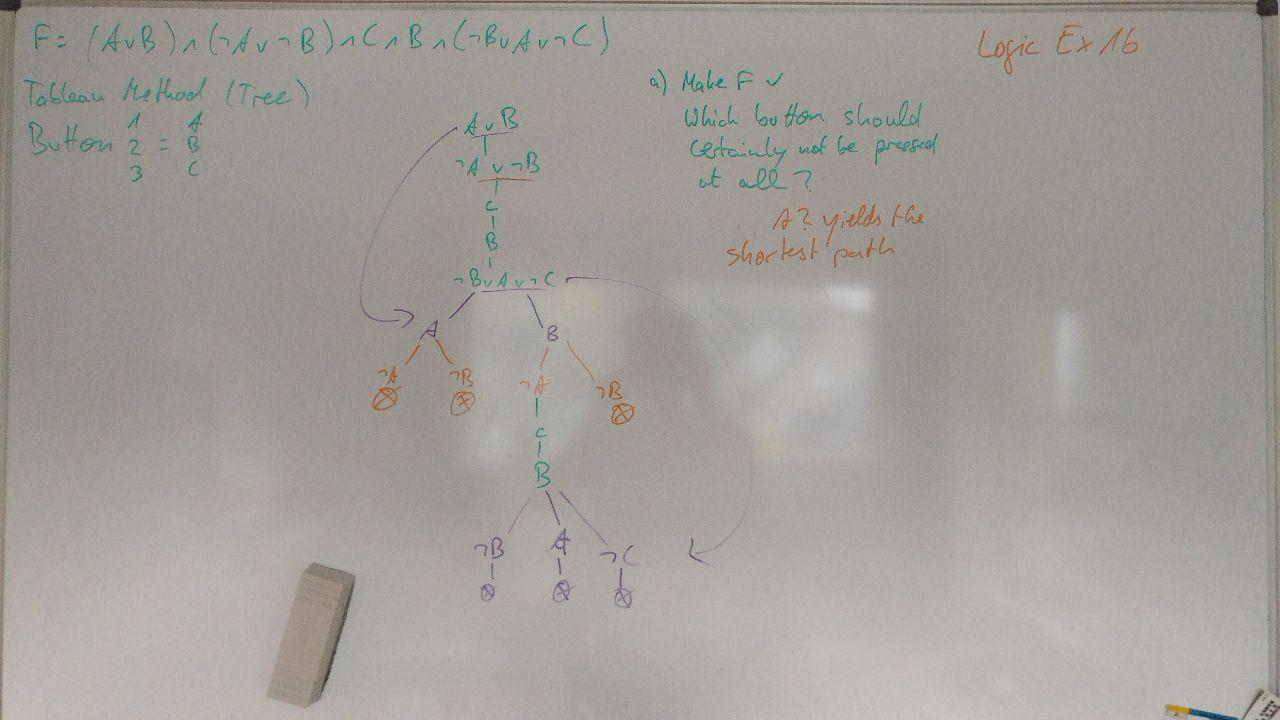
\includegraphics[scale=0.5]{../pics/ex16.jpg}
	\caption{Solution for Exercise 16 a}
\end{figure}

%ANARCHY
\end{document}